\documentclass{article}

\usepackage{listings}
\usepackage{xcolor}
\usepackage{amsmath}
\usepackage{amsthm}
\usepackage{amssymb}
\usepackage{esint}
\usepackage[parfill]{parskip}
\usepackage{hyperref}
\usepackage{floatrow}
\usepackage{minted}
\usepackage{graphicx}
\graphicspath{{./}}
\usepackage{multirow}
\usepackage{multicol}


\title{Technical Typesetting Assignment}
\author{Nitsure Omkar Milind}
\date{6th August 2022}

\begin{document}

\maketitle

\tableofcontents

\newpage

\section{Listings and Environments}

\newcounter{Listing}

\lstset{
numbers=left,
breaklines=true,
keywordstyle=\color{blue}\bfseries,
numberstyle=\tiny\color{gray},
commentstyle=\color{green!30!black},
stringstyle=\color{violet}
}


\refstepcounter{Listing}
    \begin{center}
      \textbf{\large{Listing \theListing : [LaTeX]TeX}}  \\
      \textbf{An Example}
    \end{center}
\vspace{-1em}

\begin{lstlisting}[language=Mathematica]
\Begin{lstlisting}
%A regular \lstlisting environment wont work. Youll
    have to use \lstnewenvironment to define a custom
    environment.
\End{lstlisting}
\end{lstlisting}

\vspace{2em}


\refstepcounter{Listing}
    \begin{center}
      \textbf{\large{Listing \theListing : Python}}  \\
      \textbf{Regular Stuff}
    \end{center}
\vspace{-1em}

\begin{lstlisting}[language=Python]
from scipy import *
#The custom environment you define should be numbered as
    #well.We did this in our tutorial.Think about what
    #arguments you can pass to it .
print("Hello!")
\end{lstlisting}

\vspace{2em}


\refstepcounter{Listing}
    \begin{center}
      \textbf{\large{Listing \theListing : C++}}  \\
      \textbf{Generic Title}
    \end{center}
\vspace{-1em}

\begin{lstlisting}[language=C++]
#include <iostream>
using namespace std;

//From the three examples, you must have observed what
      //you can hardcode.

int main(int argc,char* argv[])
{
     cout<<"Hello!"<<endl;
}
\end{lstlisting}

\vspace{3em}


The 2em vertical space after the listing is part of the custom environment.

\newpage


\section{Formal Logic: Figures and Tables}

\begin{figure}[H]
    \centering
    \begin{floatrow}
        \ffigbox[0.4\textwidth]{\caption{ Aristotle: The first
            formal logician.}}{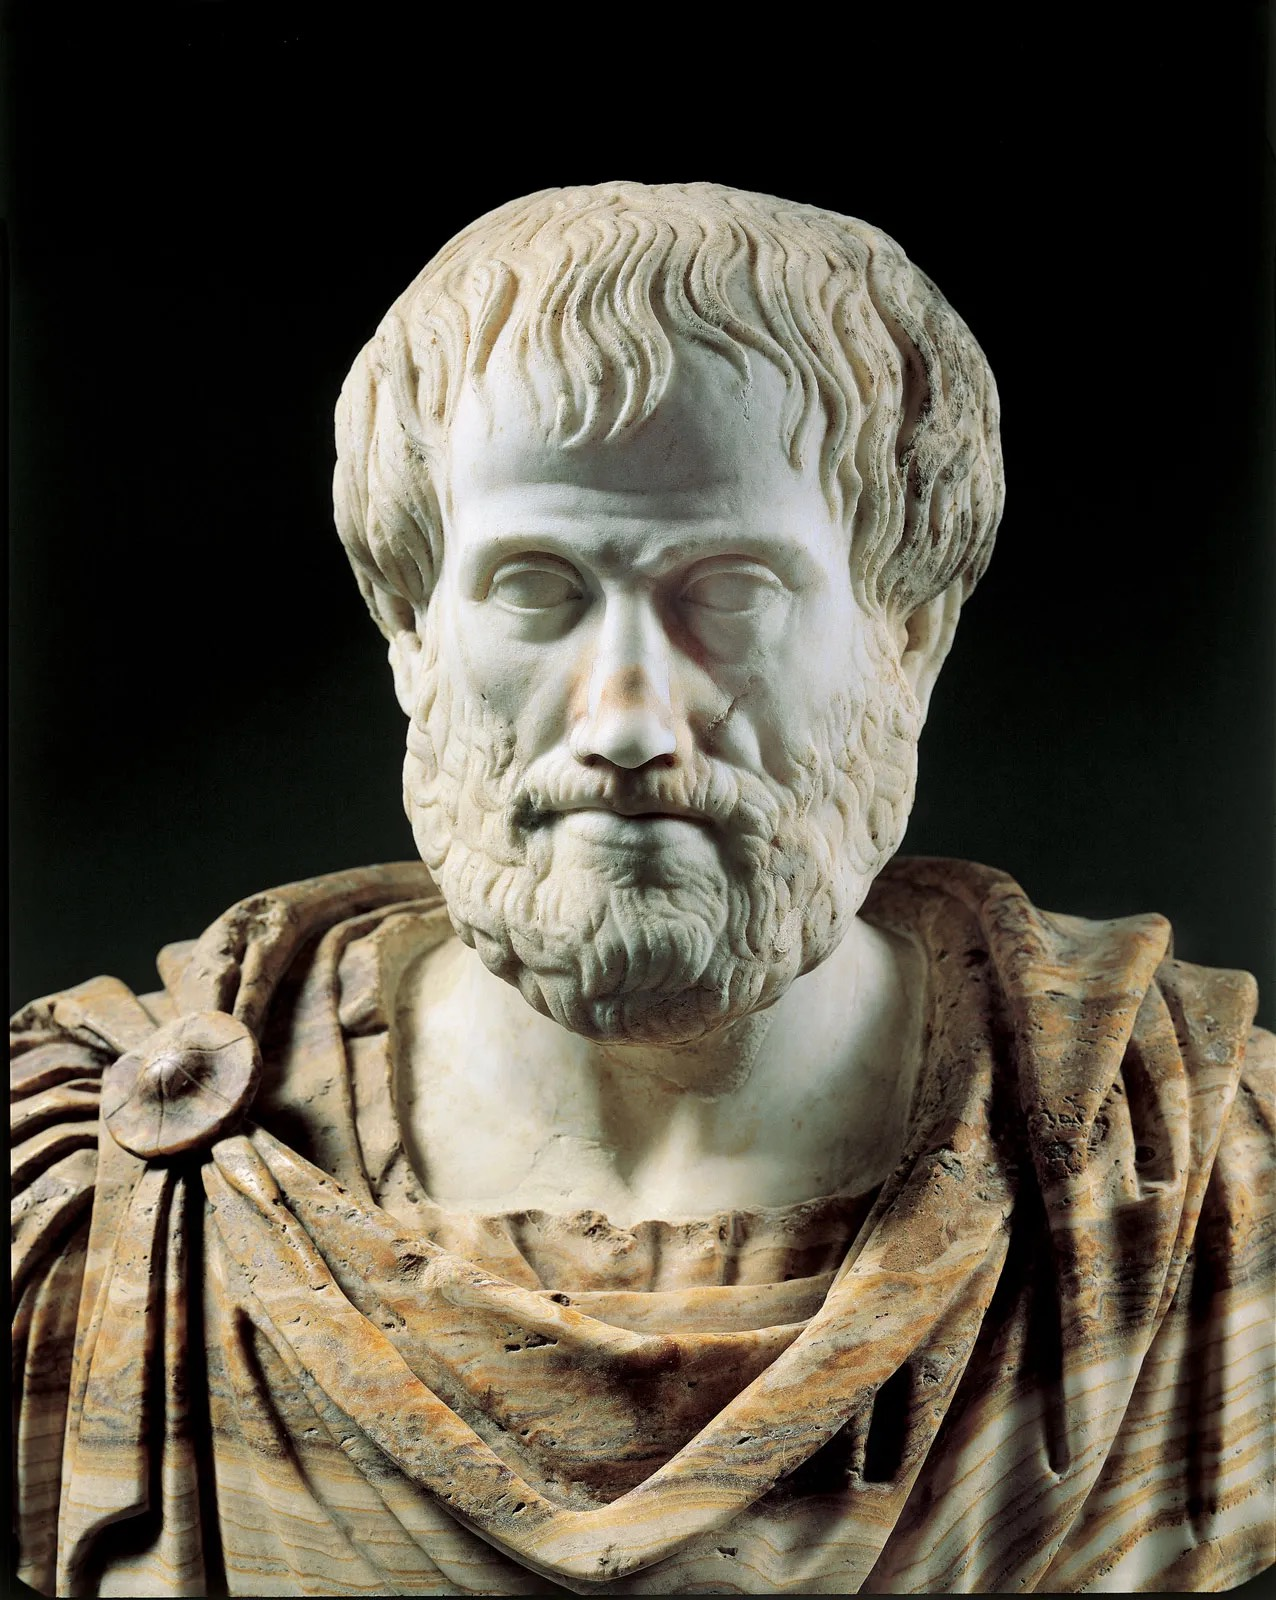
\includegraphics[width=0.4\textwidth]{aristotle.jpg}}
        \ffigbox[0.4\textwidth]{\caption{ Aristotle: The first
            formal logician.}}{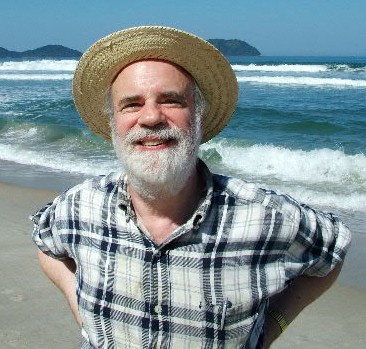
\includegraphics[width=0.52\textwidth]{saul kripke.jpg}}
    \end{floatrow}
\end{figure}

\href{https://www.britannica.com/biography/Aristotle}{Aristotle image source} \par \vspace{-0.7em}
\href{https://commons.wikimedia.org/w/index.php?curid=5763037}{Saul Kripke image source} \par

Make sure you follow these links, so you know where the hyperlinks lead to
when you typeset it yourself.

\begin{table}[H]
    \centering
    \begin{tabular}{c|c}
       \hline
       \textbf{Assertion} & \textbf{Negation} \\
       \hline
       $p(x)$ & \neg $p(x)$ \\
       \hline
       \perp & $p(x)$ \vee \neg $p(x)$ \\& \perp \\
       \hline
        $p(x)$ \wedge $q(x)$ & \neg ($p(x)$ \wedge $q(x)$) \\& \neg $p(x)$ \vee \neg $q(x)$ \\
        \hline
        \exists $x.p(x)$ & \forall $x.$ \neg $p(x)$\\
        \hline
        $p(x)$ \implies $q(x)$ & \neg (\neg $p(x)$ \vee $q(x)$) \\ & $p(x)$ \wedge \neg $q(x)$ \\
        \hline
        \multicolumn{2}{c}{This statement is false.}\\
        \hline
    \end{tabular}
    \caption{Some First Order Logic, and an absurdity.}
    \label{tab:my_label}
\end{table}

This table uses multirow as well as multicolumn. Replicate it as well as you
can.

\newpage

\section{Maths,Theorems and References}

\newtheorem{theorem}{Theorem}
\begin{theorem}[Divergence Theorem]
\begin{gather*}
    \iiint_V \ (\boldsymbol{\nabla \cdot F}) \,dV = \oiint_S (\boldsymbol{F \cdot \hat{n}}) \,dS
\end{gather*} 
Remark.\emph{You Have definitely studied and applied the theorem extensively in \\
MA 105. It also shows up as Gauss’ Law in electrodynamics.} 
\end{theorem}

\newtheorem{proposition}{Proposition}[section]

\begin{proposition}[\emph{George Cantor}]
Let $\mathbb{N}$ be the set of natural numbers. Denote its cardinality $\vert \mathbb{N} \vert$  by N.Let $\mathbb{R}$ be the set of real numbers. Its cardinality $\mathfrak{c}$ is sometimes called the cardinality of the continuum.  $\mathfrak{c} = 2^{N}$ \par
Hint. \emph{You will find the} \verb!\mathfrak! \emph{command useful to typeset the above.}
\end{proposition}

\newtheorem{lemma}{Lemma}\label{lemma1}

\begin{lemma}[Jordan Normal Form]
For every matrix M in $\mathbb{C}^{k \times k}$ having eigenvalues $\gamma_{1},...,\gamma_{k}$, with algebraic multiplicities $m_{1},...,m_{k}$ respectively, there is an invertible matrix \emph{P} and a matrix \emph{D} of the form \emph{D} = Diag\emph{(}$J_1,...,J_k$\emph{)} with each block $J_i$ bein a $m_i \times m_i$ matrix of the form \par

$J_i = \begin{bmatrix} 
\gamma_i & 1 & 0 & ... & 0 \\
0 &\gamma_i & 1 & ... & 0 \\
\vdots &\vdots & \vdots & \ddots & \vdots \\
0 & 0 & 0 & ... & 1 \\
0 & 0 & 0 & ... & \gamma_i
\end{bmatrix}$
\centering \par
\vspace{0.5em}
\raggedright
and $M = P^{-1}DP.$ Moreover, if M is an algebraic matrix, so are D and P, and
their entries can be computed from the entries of M. \par
\emph{You have certainly studied that if M is defect free, that is, algebraic and multiplicities of its eigenvalues coincide, then it is similar to a diagonal matrix.
If not, the Jordan Normal form is the next best thing. We cite \cite{textbook1} for this lemma}\par
Hint.\emph{Look at the bibliography entry for this citation. It is a book. Specify the author, publisher, title, year and edition. Our bibliography style is} \verb!plainurl!. \par
\emph{Consider the last statement of Lemma  \ref{lemma1}. (Yes, a cross reference.)
Algebraic numbers are roots of polynomials with integer coefficients. They can be found efficiently. \cite{textbook2}}\\
Hint.\emph{This citation is an article. Specify the author, year, title,
journal, volume and number.}

\end{lemma}

\begin{thebibliography}{9}
\bibitem{textbook1}
K. Hoffman and R. Kunze. Linear Algebra. Prentice-Hall, 2nd edition, 1971

\bibitem{textbook2}
V. Pan. Optimal and nearly optimal algorithms for approximating polynomial zeros. Computers & Mathematics with Applications, 31(12), 1996.

\end{thebibliography}


\end{document}
